\section{Программирование}
\subsection{Запрос 1.1}
Найти все автомобили, которые парковались в типе зоны парковки "A", у которого тревожное событие "B" и источник координат "C".
\begin{lstlisting}[style=sqlstyle, caption={Запрос 1.1}, label={lst:schema}]
SELECT DISTINCT c.car_id, c.reg_number, c.brand, c.model
FROM car c
JOIN parking_session ps ON ps.car_id = c.car_id
JOIN parking_zone pz ON pz.parking_zone_id = ps.parking_zone_id
JOIN parking_zone_type pzt ON pzt.zone_type_id = pz.zone_type_id
JOIN alert_event ae ON ae.car_id = c.car_id
JOIN alert_event_type aet ON aet.alert_event_type_id = ae.alert_event_type_id
JOIN track t ON t.car_id = c.car_id
JOIN track_point tp ON tp.track_id = t.track_id
JOIN data_source_type dst ON dst.data_source_id = tp.data_source_id
WHERE pzt.name = 'Бесплатная'
  AND aet.name = 'Потеря связи'
  AND dst.name = 'GPS';
\end{lstlisting}

\begin{figure}[H]
    \centering
    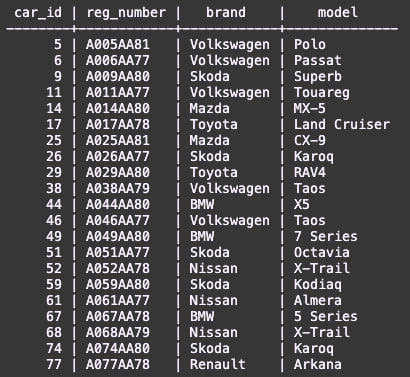
\includegraphics[width=0.69\linewidth]{myPhoto/1.1.jpg}
    \caption{Результат выполнения запроса 1.1}
    \label{fig:req11}
\end{figure}

\begin{figure}[H]
    \centering
    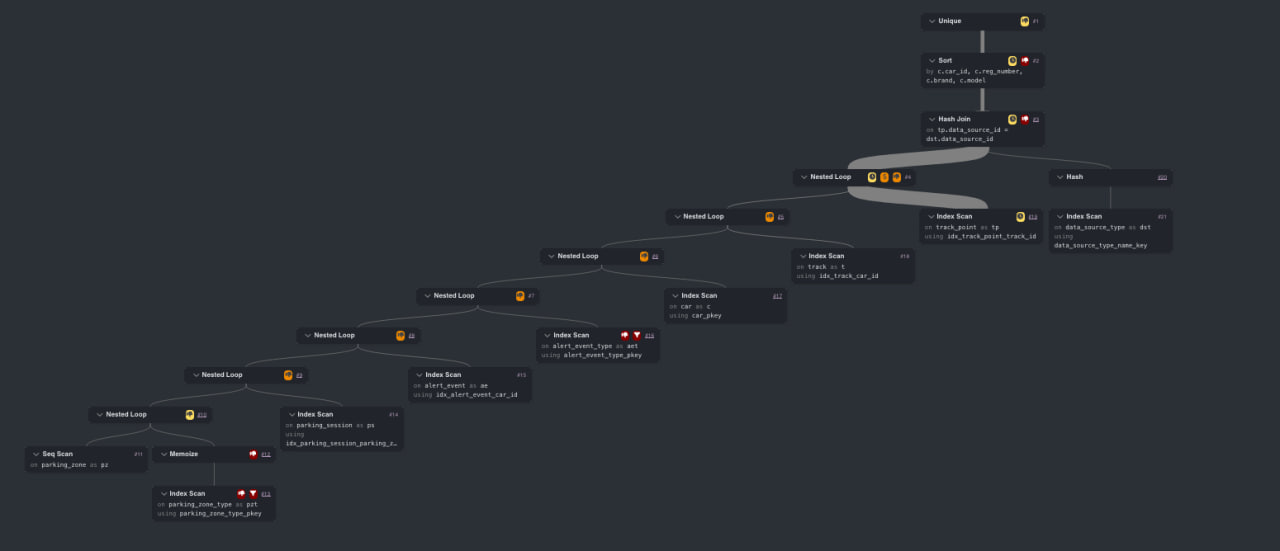
\includegraphics[width=0.69\linewidth]{myPhoto/1.1.query.jpg}
    \caption{План выполнения запроса 1.1}
    \label{fig:query11}
\end{figure}

Время выполнения запроса: \\
Planning Time: 3.444 ms \\
Execution Time: 248.770 ms \\


\newpage


\subsection{Запрос 1.2}
Найти все автомобили, которые парковались в типе зоны парковки "A", у которого тревожное событие "B" и источник координат "C", не менее 3 раз.
\begin{lstlisting}[style=sqlstyle, caption={Запрос 1.2}, label={lst:req12}]
SELECT c.car_id, c.reg_number, c.brand, c.model,
       COUNT(DISTINCT ps.parking_session_id) AS cnt
FROM car c
JOIN parking_session ps ON ps.car_id = c.car_id
JOIN parking_zone pz ON pz.parking_zone_id = ps.parking_zone_id
JOIN parking_zone_type pzt ON pzt.zone_type_id = pz.zone_type_id
JOIN alert_event ae ON ae.car_id = c.car_id
JOIN alert_event_type aet ON aet.alert_event_type_id = ae.alert_event_type_id
JOIN track t ON t.car_id = c.car_id
JOIN track_point tp ON tp.track_id = t.track_id
JOIN data_source_type dst ON dst.data_source_id = tp.data_source_id
WHERE pzt.name = 'Бесплатная'
  AND aet.name = 'Потеря связи'
  AND dst.name = 'GPS'
GROUP BY c.car_id, c.reg_number, c.brand, c.model
HAVING COUNT(DISTINCT ps.parking_session_id) >= 3;
\end{lstlisting}

\begin{figure}[H]
    \centering
    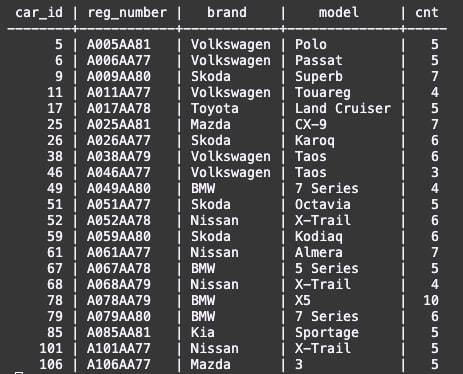
\includegraphics[width=0.69\linewidth]{myPhoto/1.2.jpg}
    \caption{Результат выполнения запроса 1.2}
    \label{fig:req12}
\end{figure}

\begin{figure}[H]
    \centering
    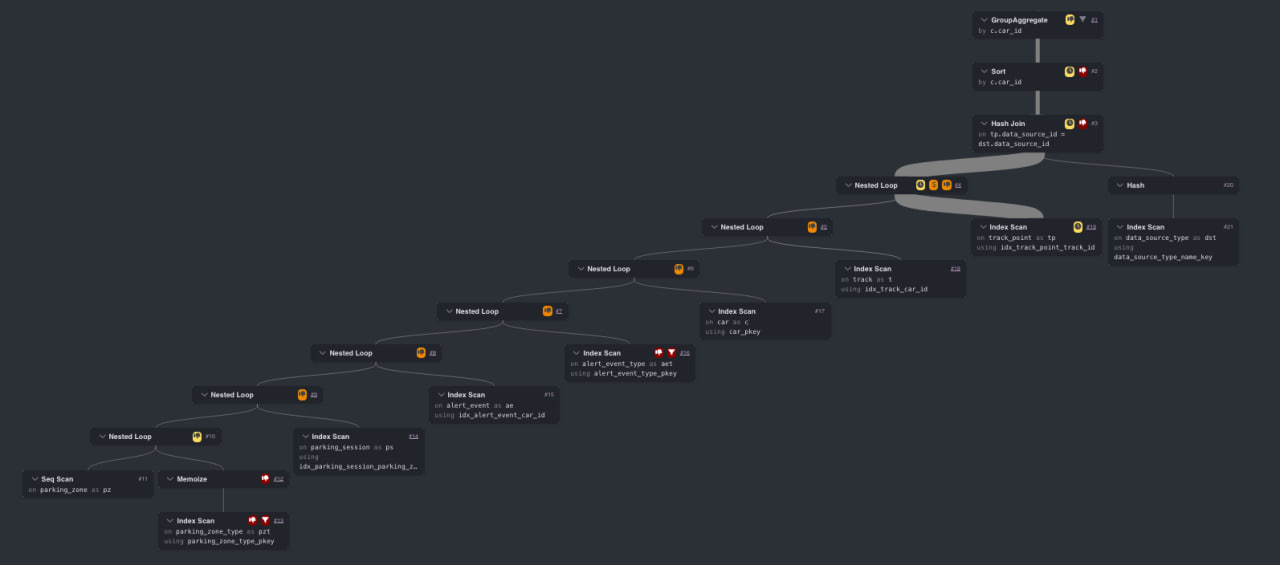
\includegraphics[width=0.69\linewidth]{myPhoto/1.2.query.jpg}
    \caption{План выполнения запроса 1.2}
    \label{fig:query12}
\end{figure}

Время выполнения запроса: \\
Planning Time: 2.730 ms \\
Execution Time: 113.795 ms \\


\newpage


\subsection{Запрос 2}
Для сотрудника "А", который обрабатывал тревожные события, посчитать число автомобилей, которые парковались в зоне парковки "B".
\begin{lstlisting}[style=sqlstyle, caption={Запрос 2}, label={lst:req2}]
SELECT COUNT(DISTINCT ps.car_id) AS car_count
FROM parking_session ps
JOIN parking_zone pz ON pz.parking_zone_id = ps.parking_zone_id
WHERE pz.name = 'ТЦ Мега — парковка В'
  AND ps.car_id IN (
      SELECT ae.car_id
      FROM alert_event ae
      JOIN employee e ON e.employee_id = ae.employee_id
      WHERE e.full_name = 'Иванов Игорь Николаевич'
  );
\end{lstlisting}

\begin{figure}[H]
    \centering
    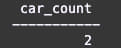
\includegraphics[width=0.69\linewidth]{myPhoto/2.jpg}
    \caption{Результат выполнения запроса 2}
    \label{fig:req2}
\end{figure}

\begin{figure}[H]
    \centering
    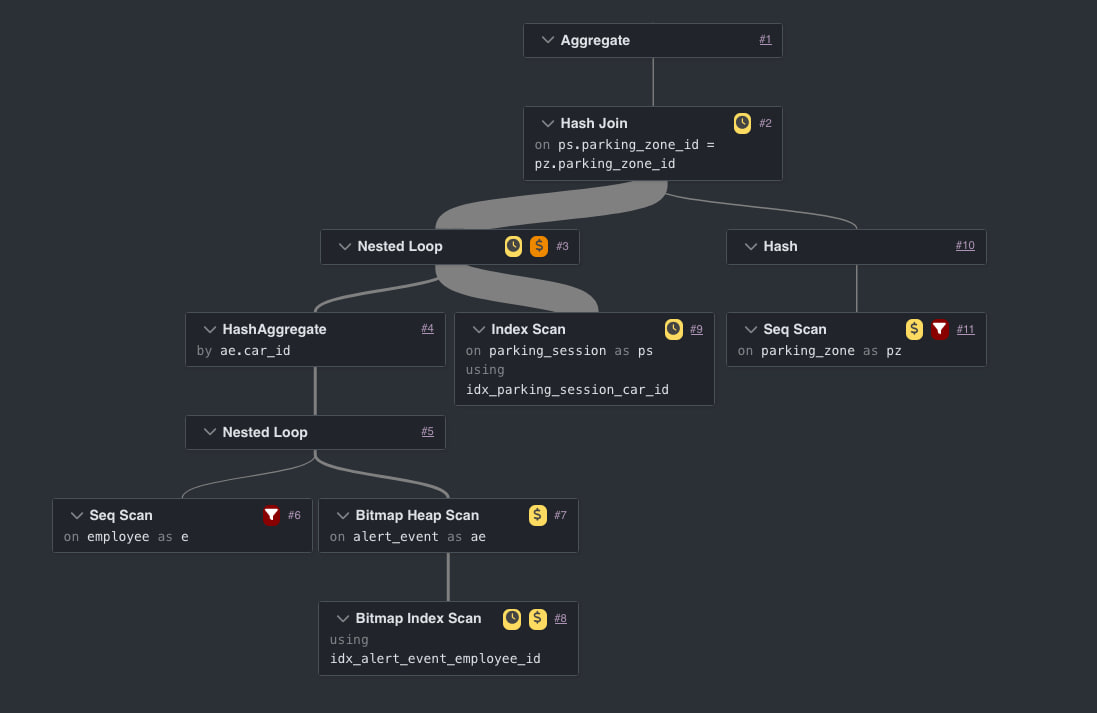
\includegraphics[width=0.69\linewidth]{myPhoto/2.query.jpg}
    \caption{План выполнения запроса 2}
    \label{fig:query2}
\end{figure}

Время выполнения запроса: \\
Planning Time: 0.427 ms \\
Execution Time: 0.166 ms \\

\newpage


\subsection{Запрос 3}
Для каждого сотрудника посчитать число тревожных событий и количество автомобилей.
\begin{lstlisting}[style=sqlstyle, caption={Запрос 3}, label={lst:req3}]
SELECT e.employee_id, e.full_name,
       COUNT(DISTINCT ae.alert_event_id) AS alert_count,
       COUNT(DISTINCT ae.car_id) AS car_count
FROM employee e
LEFT JOIN alert_event ae ON ae.employee_id = e.employee_id
GROUP BY e.employee_id, e.full_name
ORDER BY e.employee_id;
\end{lstlisting}

\begin{figure}[H]
    \centering
    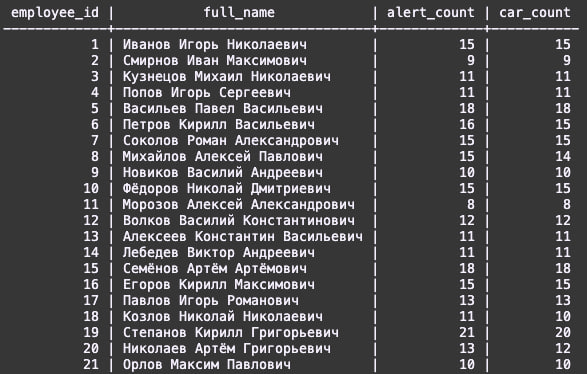
\includegraphics[width=0.69\linewidth]{myPhoto/3.jpg}
    \caption{Результат выполнения запроса 3}
    \label{fig:req3}
\end{figure}

\begin{figure}[H]
    \centering
    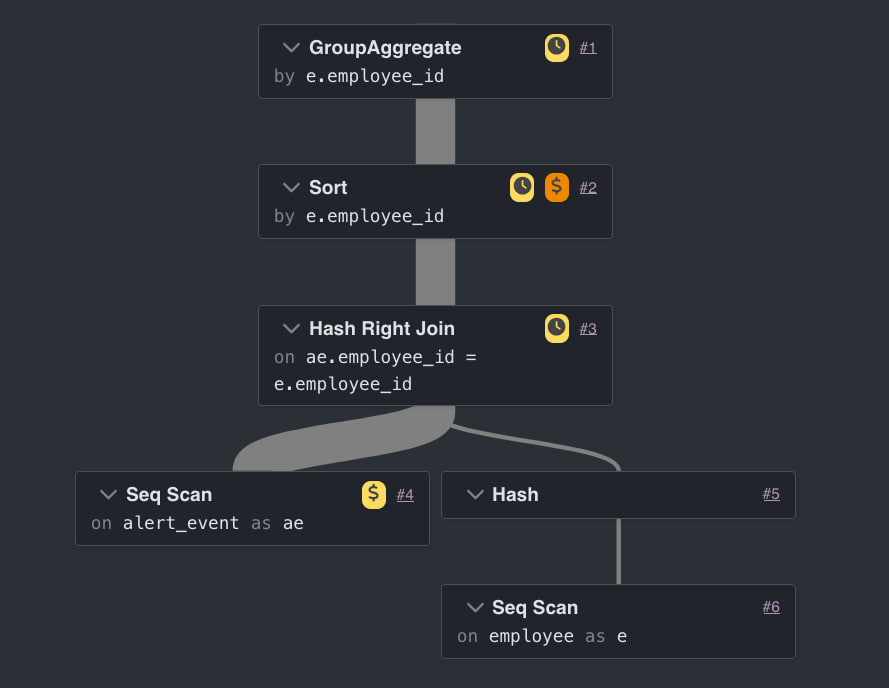
\includegraphics[width=0.69\linewidth]{myPhoto/3.query.jpg}
    \caption{План выполнения запроса 3}
    \label{fig:query3}
\end{figure}

\begin{figure}[H]
    \centering
    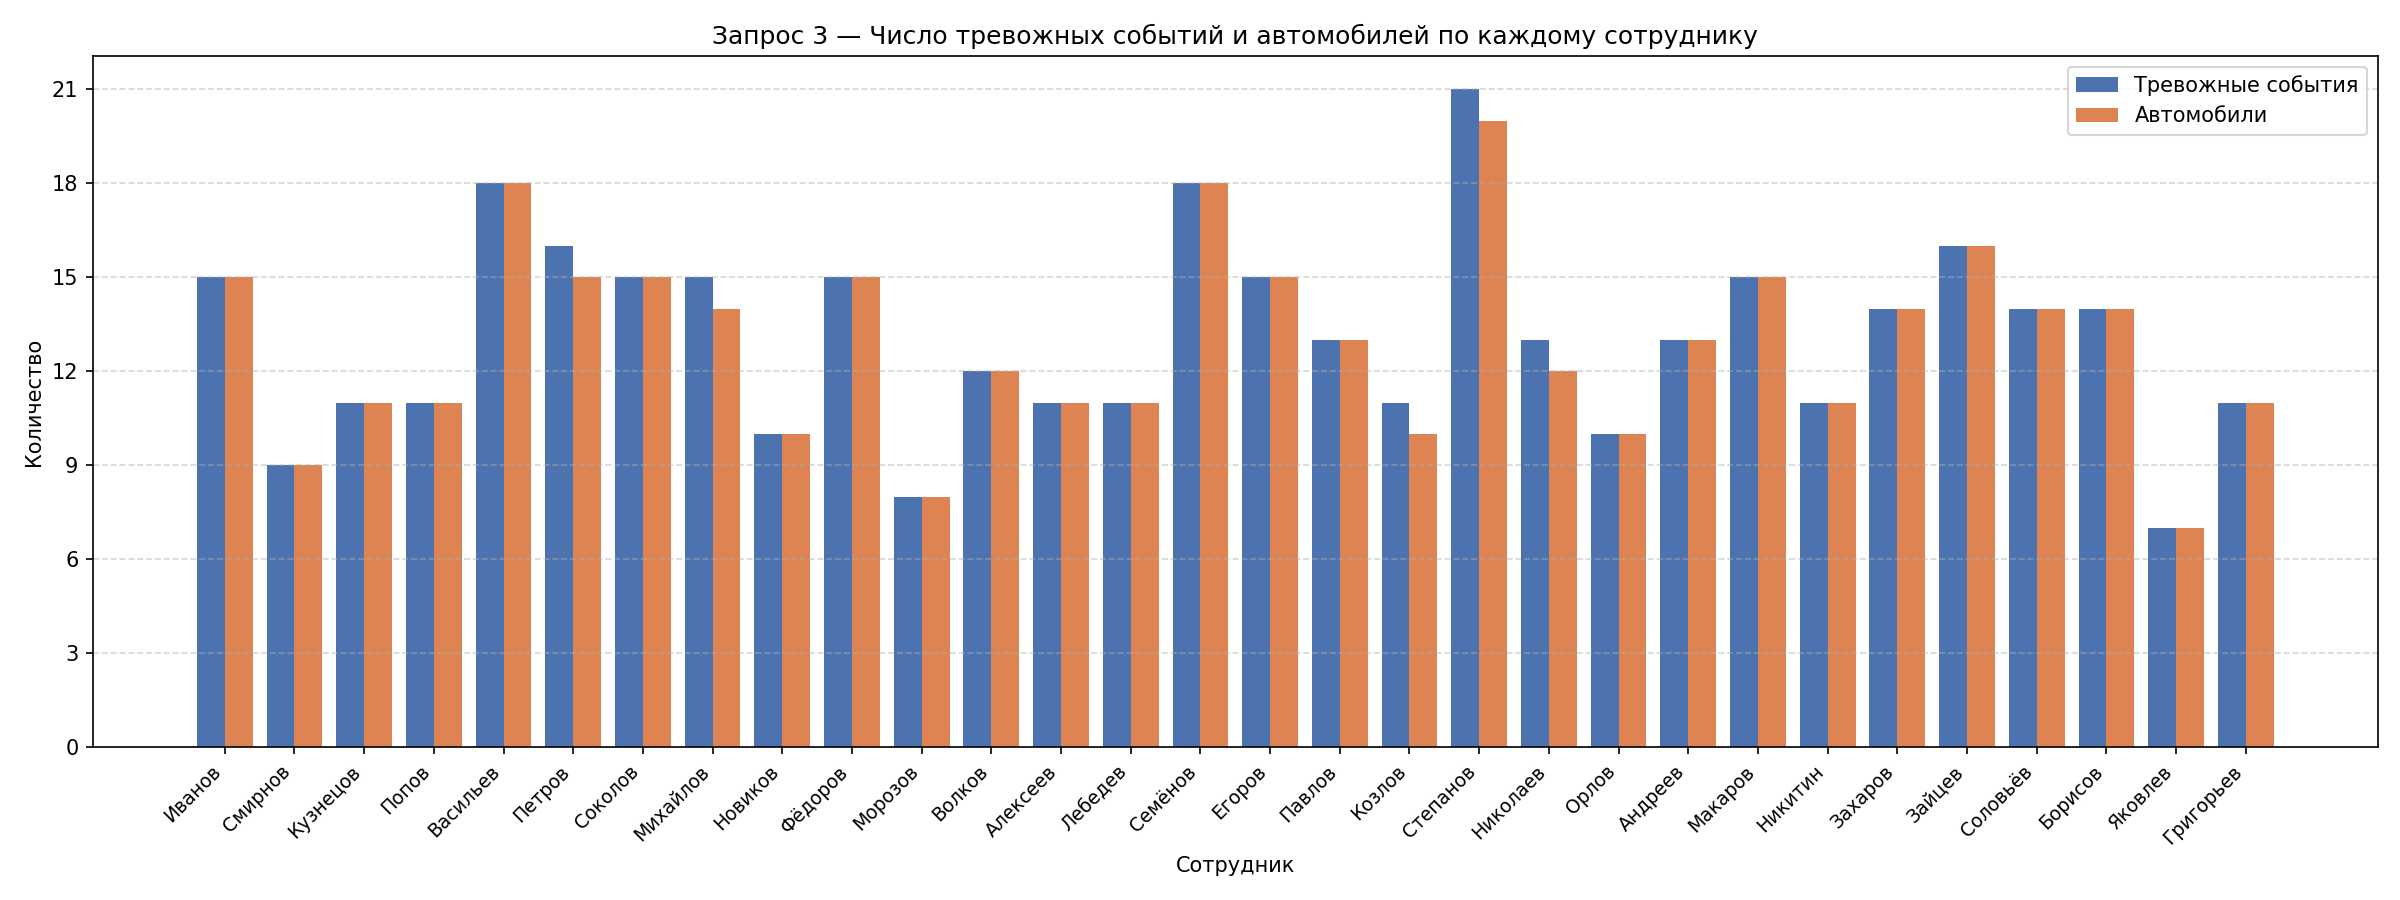
\includegraphics[width=\linewidth]{myPhoto/hist3.png}
    \caption{Гистограмма запроса 3 — число тревожных событий и автомобилей по каждому сотруднику}
    \label{fig:hist3}
\end{figure}

Время выполнения запроса: \\
Planning Time: 0.288 ms \\
Execution Time: 0.297 ms \\

\newpage


\subsection{Запрос 4}
\begin{itemize}
	\item Найти зоны парковки в которых парковалось максимальное количество автомобилей.
	\item Найти зоны парковки в которых парковалось минимальное количество автомобилей.
\end{itemize}
\begin{lstlisting}[style=sqlstyle, caption={Запрос 4 min/max}, label={lst:req4}]
-- MAX
SELECT pz.parking_zone_id, pz.name, COUNT(DISTINCT ps.car_id) AS cnt
FROM parking_zone pz
JOIN parking_session ps ON ps.parking_zone_id = pz.parking_zone_id
GROUP BY pz.parking_zone_id, pz.name
HAVING COUNT(DISTINCT ps.car_id) = (
    SELECT MAX(sub.car_count)
    FROM (
        SELECT COUNT(DISTINCT ps2.car_id) AS car_count
        FROM parking_session ps2
        GROUP BY ps2.parking_zone_id
    ) sub
);

-- MIN
SELECT pz.parking_zone_id, pz.name, COUNT(DISTINCT ps.car_id) AS cnt
FROM parking_zone pz
JOIN parking_session ps ON ps.parking_zone_id = pz.parking_zone_id
GROUP BY pz.parking_zone_id, pz.name
HAVING COUNT(DISTINCT ps.car_id) = (
    SELECT MIN(sub.car_count)
    FROM (
        SELECT COUNT(DISTINCT ps2.car_id) AS car_count
        FROM parking_session ps2
        GROUP BY ps2.parking_zone_id
    ) sub
);
\end{lstlisting}

\begin{figure}[H]
    \centering
    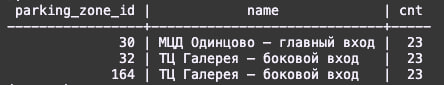
\includegraphics[width=0.69\linewidth]{myPhoto/4_max.jpg}
    \caption{Результат выполнения запроса 4 (макс)}
    \label{fig:req4max}
\end{figure}

\begin{figure}[H]
    \centering
    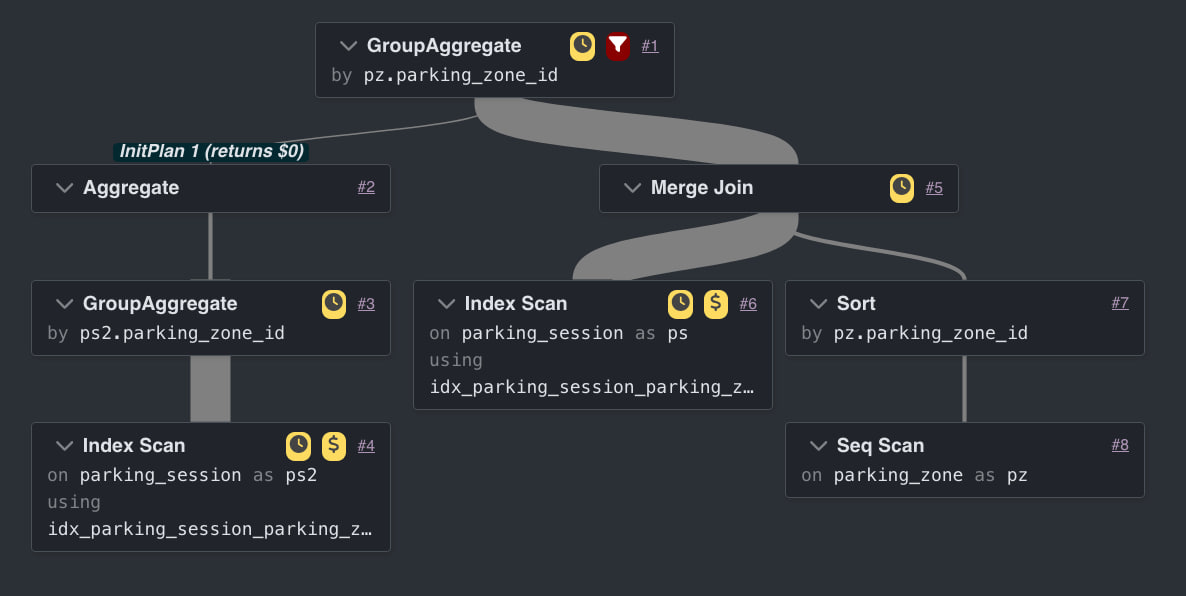
\includegraphics[width=0.69\linewidth]{myPhoto/4_max.query.jpg}
    \caption{План выполнения запроса 4 (макс)}
    \label{fig:query4max}
\end{figure}

Время выполнения запроса (макс): \\
Planning Time: 0.419 ms \\
Execution Time: 1.743 ms \\

\begin{figure}[H]
    \centering
    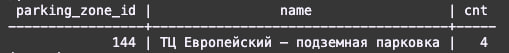
\includegraphics[width=0.69\linewidth]{myPhoto/4_min.jpg}
    \caption{Результат выполнения запроса 4 (мин)}
    \label{fig:req4min}
\end{figure}

\begin{figure}[H]
    \centering
    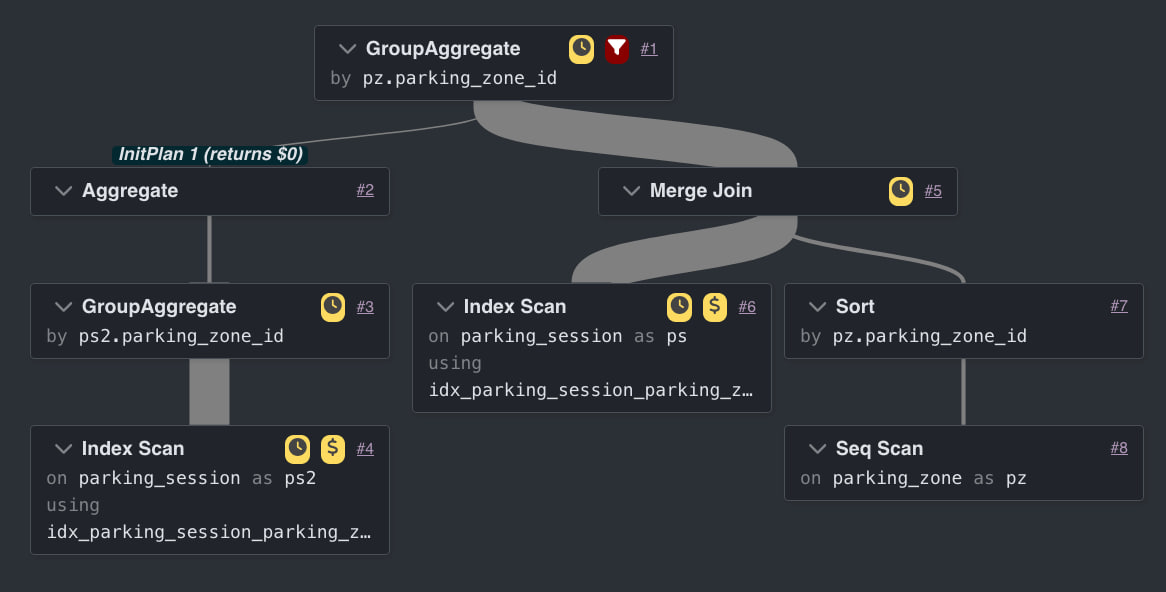
\includegraphics[width=0.69\linewidth]{myPhoto/4_min.query.jpg}
    \caption{План выполнения запроса 4 (мин)}
    \label{fig:query4min}
\end{figure}

Время выполнения запроса (мин): \\
Planning Time: 0.335 ms \\
Execution Time: 1.449 ms \\

\newpage


\subsection{Запрос 5}
Найти число зон парковок, с одинаковых числом паркововавшихся автомобилей для каждого сотрудника.
\begin{lstlisting}[style=sqlstyle, caption={Запрос 5}, label={lst:req5}]
SELECT e.full_name, sub.car_count, COUNT(*) AS zone_count
FROM employee e
JOIN (
    SELECT ae.employee_id, ps.parking_zone_id,
           COUNT(DISTINCT ae.car_id) AS car_count
    FROM alert_event ae
    JOIN parking_session ps ON ps.car_id = ae.car_id
    GROUP BY ae.employee_id, ps.parking_zone_id
) sub ON sub.employee_id = e.employee_id
GROUP BY e.full_name, sub.car_count
ORDER BY e.full_name, sub.car_count;
\end{lstlisting}

\begin{figure}[H]
    \centering
    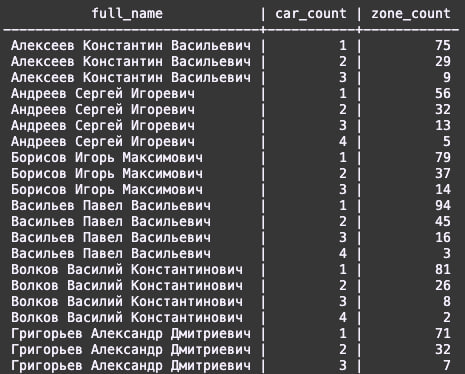
\includegraphics[width=0.69\linewidth]{myPhoto/5.jpg}
    \caption{Результат выполнения запроса 5}
    \label{fig:req5}
\end{figure}

\begin{figure}[H]
    \centering
    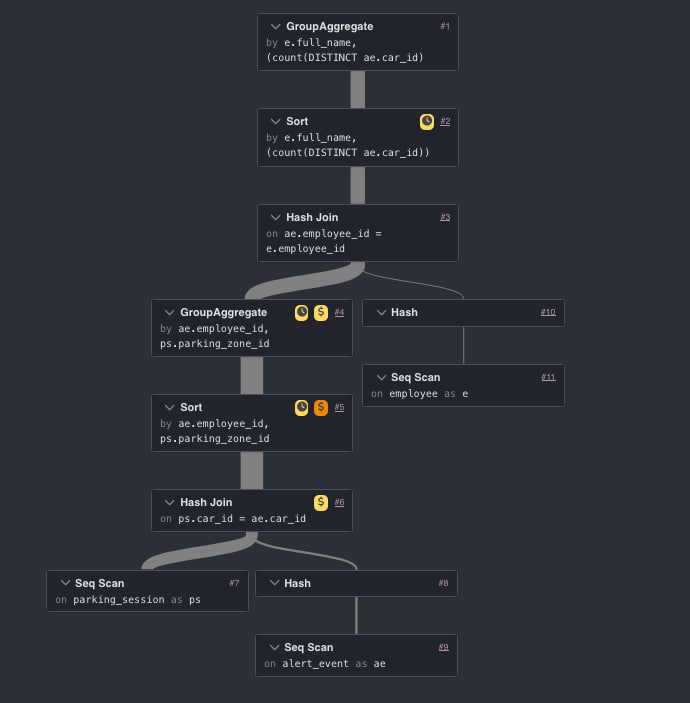
\includegraphics[width=0.69\linewidth]{myPhoto/5.query.jpg}
    \caption{План выполнения запроса 5}
    \label{fig:query5}
\end{figure}

\clearpage
\newgeometry{paperwidth=430mm,paperheight=297mm,margin=-2mm}
\begin{landscape}
  \thispagestyle{empty}
  \captionsetup{font=small,skip=4pt}

  \begin{figure}[!p]
    \centering
    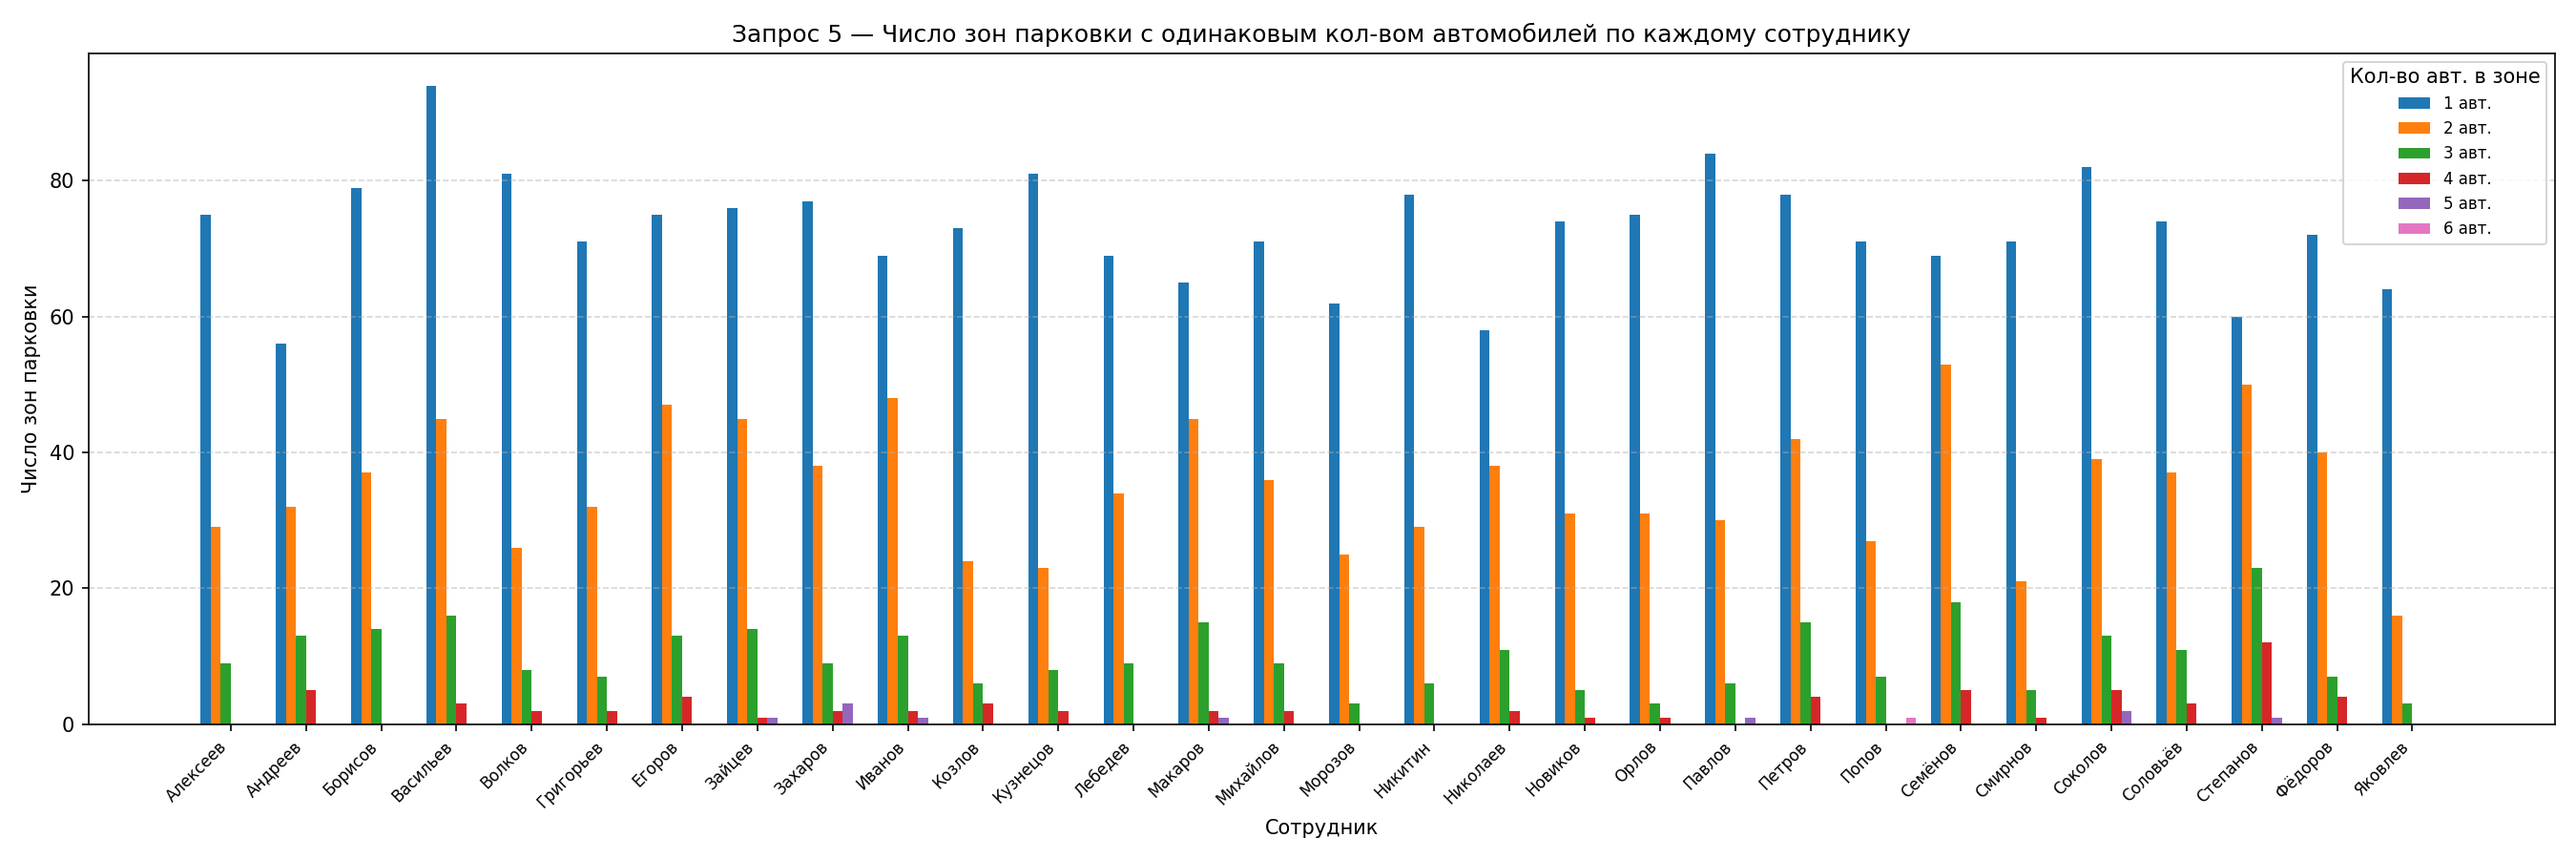
\includegraphics[width=\linewidth,height=\dimexpr\textheight-4\baselineskip\relax,keepaspectratio]{myPhoto/hist5.png}
    \caption{Гистограмма запроса 5 — число зон парковки с одинаковым количеством автомобилей по каждому сотруднику}
    \label{fig:hist5}
  \end{figure}
\end{landscape}
\restoregeometry
\clearpage

Время выполнения запроса: \\
Planning Time: 0.437 ms \\
Execution Time: 4.812 ms \\

\newpage

\subsection{Запрос 6}
Найти сотрудников, которые обработали больше тревожных событий, чем сотрудник "A".
\begin{lstlisting}[style=sqlstyle, caption={Запрос 6}, label={lst:req6}]
SELECT e.employee_id, e.full_name, COUNT(ae.alert_event_id) AS cnt
FROM employee e
JOIN alert_event ae ON ae.employee_id = e.employee_id
GROUP BY e.employee_id, e.full_name
HAVING COUNT(ae.alert_event_id) > (
    SELECT COUNT(ae2.alert_event_id)
    FROM alert_event ae2
    JOIN employee e2 ON e2.employee_id = ae2.employee_id
    WHERE e2.full_name = 'Иванов Игорь Николаевич'
)
ORDER BY cnt DESC;
\end{lstlisting}

\begin{figure}[H]
    \centering
    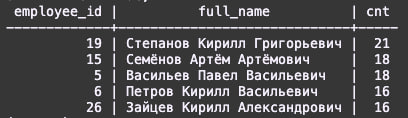
\includegraphics[width=0.69\linewidth]{myPhoto/6.jpg}
    \caption{Результат выполнения запроса 6}
    \label{fig:req6}
\end{figure}

\begin{figure}[H]
    \centering
    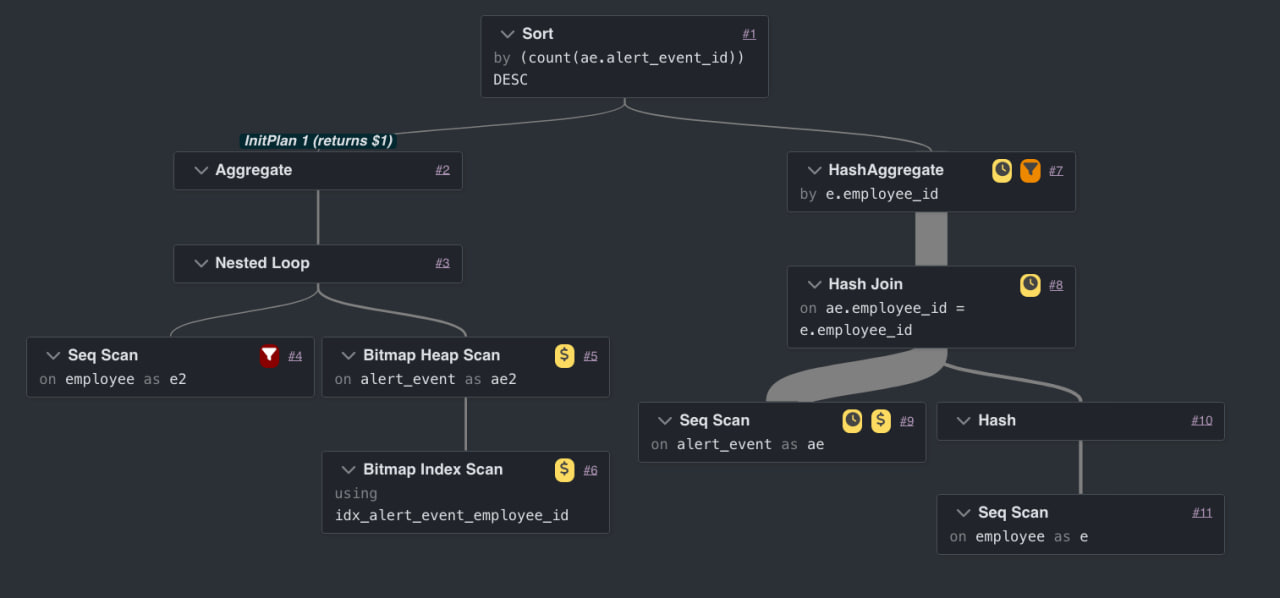
\includegraphics[width=0.69\linewidth]{myPhoto/6.query.jpg}
    \caption{План выполнения запроса 6}
    \label{fig:query6}
\end{figure}

Время выполнения запроса: \\
Planning Time: 0.331 ms \\
Execution Time: 0.217 ms \\

\newpage

\subsection{Запрос 7}
Найти зоны парковки, в которых никогда не парковался автомобиль "A".
\begin{lstlisting}[style=sqlstyle, caption={Запрос 7}, label={lst:req7}]
SELECT pz.parking_zone_id, pz.name
FROM parking_zone pz
WHERE pz.parking_zone_id NOT IN (
    SELECT ps.parking_zone_id
    FROM parking_session ps
    JOIN car c ON c.car_id = ps.car_id
    WHERE c.reg_number = 'А001АА77'
);
\end{lstlisting}

\begin{figure}[H]
    \centering
    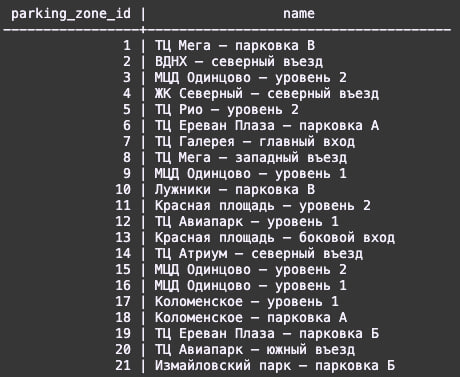
\includegraphics[width=0.69\linewidth]{myPhoto/7.jpg}
    \caption{Результат выполнения запроса 7}
    \label{fig:req7}
\end{figure}

\begin{figure}[H]
    \centering
    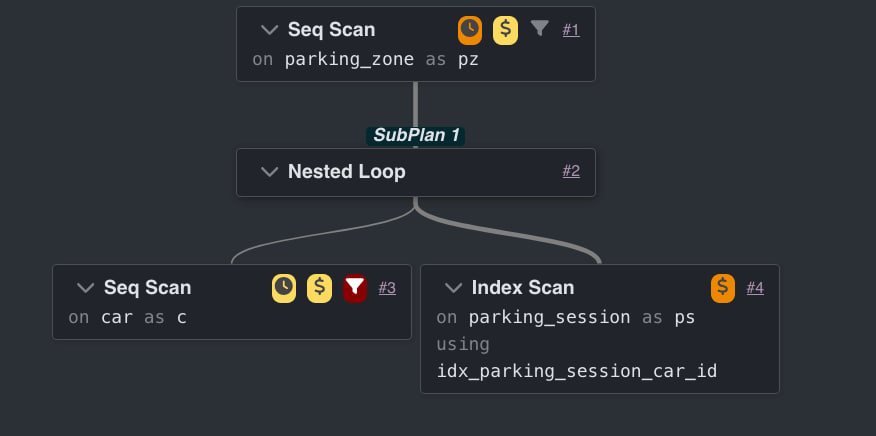
\includegraphics[width=0.69\linewidth]{myPhoto/7.query.jpg}
    \caption{План выполнения запроса 7}
    \label{fig:query7}
\end{figure}

Время выполнения запроса: \\
Planning Time: 0.403 ms \\
Execution Time: 0.100 ms \\

\newpage

\subsection{Запрос 8}
Для каждого источника данных, автомобилей, посчитать количество координат.
\begin{lstlisting}[style=sqlstyle, caption={Запрос 8}, label={lst:req8}]
SELECT c.car_id, c.reg_number, dst.name AS data_source,
       COUNT(tp.track_point_id) AS coord_count
FROM data_source_type dst
JOIN track_point tp ON tp.data_source_id = dst.data_source_id
JOIN car c ON c.car_id = tp.car_id
GROUP BY c.car_id, c.reg_number, dst.data_source_id, dst.name
ORDER BY c.car_id, dst.name;
\end{lstlisting}

\begin{figure}[H]
    \centering
    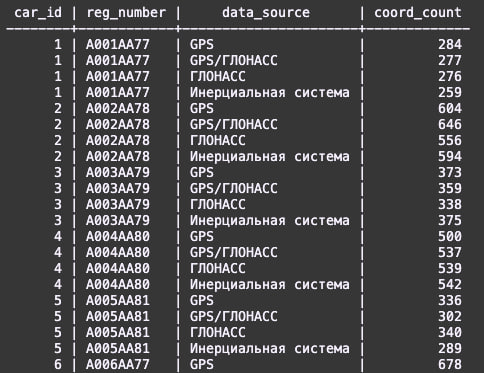
\includegraphics[width=0.69\linewidth]{myPhoto/8.jpg}
    \caption{Результат выполнения запроса 8}
    \label{fig:req8}
\end{figure}

\begin{figure}[H]
    \centering
    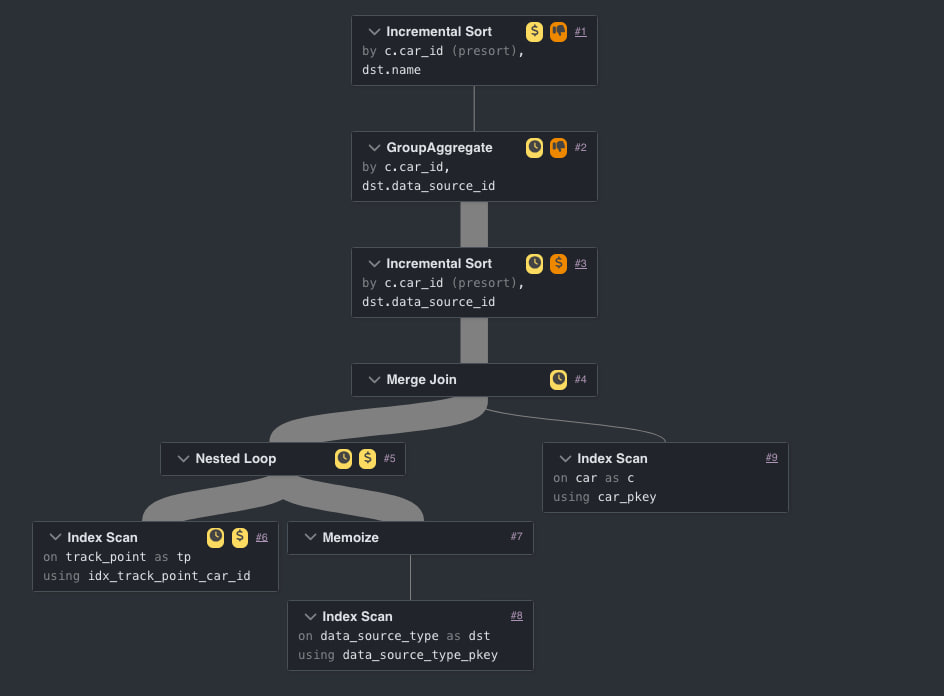
\includegraphics[width=0.69\linewidth]{myPhoto/8.query.jpg}
    \caption{План выполнения запроса 8}
    \label{fig:query8}
\end{figure}

\clearpage
\newgeometry{paperwidth=430mm,paperheight=297mm,margin=-2mm}
\begin{landscape}
  \thispagestyle{empty}
  \captionsetup{font=small,skip=4pt}

  \begin{figure}[!p]
    \centering
    
\includegraphics[width=\linewidth,height=\dimexpr\textheight-4\baselineskip\relax,keepaspectratio]{myPhoto/hist8.png}
    \caption{3D-гистограмма запроса 8 — количество координат по автомобилю и источнику данных}
    \label{fig:hist8}
  \end{figure}
\end{landscape}
\restoregeometry
\clearpage

Время выполнения запроса: \\
Planning Time: 0.432 ms \\
Execution Time: 139.903 ms \\

\newpage

\subsection{Запрос 9}
Для всех треков автомобиля "А", поменять статус трека с "A" на "B".
\begin{lstlisting}[style=sqlstyle, caption={Запрос 9}, label={lst:req9}]
UPDATE track
SET track_status_id = (
    SELECT track_status_id FROM track_status_type WHERE name = 'Завершён'
)
WHERE car_id = (SELECT car_id FROM car WHERE reg_number = 'А001АА77')
  AND track_status_id = (
    SELECT track_status_id FROM track_status_type WHERE name = 'Активный'
  );
\end{lstlisting}

\begin{figure}[H]
    \centering
    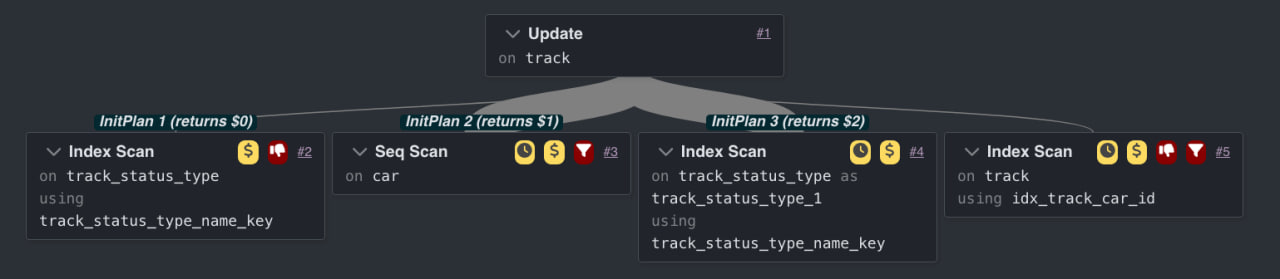
\includegraphics[width=0.69\linewidth]{myPhoto/9.query.jpg}
    \caption{План выполнения запроса 9}
    \label{fig:query9}
\end{figure}

Время выполнения запроса: \\
Planning Time: 0.266 ms \\
Execution Time: 0.078 ms \\


\newpage
